\documentclass[10pt,a4paper]{article}

\usepackage[T1]{fontenc}
\usepackage[utf8]{inputenc}
\usepackage{lmodern}
\usepackage{geometry}
\usepackage{microtype}
\usepackage{amsmath,amssymb,bm}
\usepackage{booktabs,longtable,tabularx,array}
\usepackage{xcolor}
\usepackage{graphicx}
\usepackage{tikz}
\usetikzlibrary{arrows.meta,positioning,calc,fit,shapes.geometric}
\usepackage{pgfplots}
\usepgfplotslibrary{groupplots}
\pgfplotsset{compat=1.18}
\usepackage{enumitem}
\usepackage{float}
\usepackage{caption}
\usepackage{fancyhdr}
\usepackage{url}
\usepackage[colorlinks=true,linkcolor=DeepBlue,citecolor=DeepBlue,
            urlcolor=Teal]{hyperref}
\usepackage[capitalise,noabbrev]{cleveref}

\geometry{left=20mm,right=20mm,top=22mm,bottom=23mm}
\setlength{\parindent}{0pt}
\setlength{\parskip}{5pt}
\setlist{nosep,leftmargin=5mm}
\renewcommand{\arraystretch}{1.18}

\definecolor{DeepNavy}{HTML}{17324D}
\definecolor{DeepBlue}{HTML}{236FA1}
\definecolor{Teal}{HTML}{16837A}
\definecolor{Amber}{HTML}{C56A00}
\definecolor{Critical}{HTML}{A13D35}
\definecolor{SoftBlue}{HTML}{EAF2F8}
\definecolor{SoftTeal}{HTML}{E8F4F1}
\definecolor{SoftAmber}{HTML}{FFF2DE}
\definecolor{SoftRed}{HTML}{FBEAE8}
\definecolor{Ink}{HTML}{263238}
\definecolor{MidGray}{HTML}{65727C}
\definecolor{LightGray}{HTML}{EDF0F2}

\color{Ink}
\hypersetup{
  pdftitle={multipgs: Theory, Methods, and Technical Review},
  pdfauthor={Technical review for the multipgs package},
  pdfsubject={Theory, implementation, documentation, benchmarks, and packaging},
  pdfkeywords={polygenic score, multi-PGS, elastic net, summary statistics,
               selection index, technical review}
}

\pagestyle{fancy}
\fancyhf{}
\fancyhead[L]{\small\textcolor{MidGray}{multipgs technical review}}
\fancyhead[R]{\small\textcolor{MidGray}{v0.3.0 / 0ce9ad8}}
\fancyfoot[C]{\small\textcolor{MidGray}{\thepage}}
\renewcommand{\headrulewidth}{0.3pt}

\captionsetup{font=small,labelfont={bf,color=DeepNavy}}
\newcommand{\pkg}[1]{\texttt{#1}}
\newcommand{\code}[1]{\texttt{#1}}
\newcommand{\Rtwo}{\(R^2\)}
\newcommand{\statusbox}[2]{%
  \begin{center}
  \fcolorbox{#1}{white}{\begin{minipage}{0.92\linewidth}
  \textbf{\textcolor{#1}{#2}}
  \end{minipage}}
  \end{center}}
\newcommand{\finding}[2]{\textbf{\textcolor{#1}{#2}}}
\newcolumntype{Y}{>{\raggedright\arraybackslash}X}
\newcolumntype{L}[1]{>{\raggedright\arraybackslash}p{#1}}

\begin{document}

\hypersetup{pageanchor=false}
\begin{titlepage}
\begin{tikzpicture}[remember picture,overlay]
  \fill[DeepNavy] (current page.north west)
    rectangle ([yshift=-102mm]current page.north east);
  \fill[Teal] ([yshift=-102mm]current page.north west)
    rectangle ([yshift=-107mm]current page.north east);
\end{tikzpicture}

\vspace*{19mm}
{\color{white}\sffamily
{\Large TECHNICAL REVIEW\par}
\vspace{8mm}
{\fontsize{30}{34}\selectfont\bfseries multipgs\par}
\vspace{3mm}
{\fontsize{19}{23}\selectfont Theory, methods, evidence, and documentation\par}
}

\vspace{49mm}
\begin{tabularx}{\linewidth}{@{}L{38mm}Y@{}}
\toprule
\textbf{Reviewed state} & Package version 0.3.0, commit
\code{0ce9ad8888356dc5834f5e8c323621765ac7afb3} \\
\textbf{Review date} & 12 August 2026 \\
\textbf{Scope} & Mathematical theory, three fitting routes, implementation
contracts, checked-in benchmarks, user documentation, tests, and distribution
packaging \\
\textbf{Test baseline} & 294 tests passed on Python 3.12.13, NumPy 2.5.2,
scikit-learn 1.9.0, pytest 9.1.1, and local ldpred3 0.4.6 \\
\textbf{Artifact status} & This report is descriptive and diagnostic. It is
not a clinical validation, regulatory assessment, or substitute for
independent outcome evaluation. \\
\bottomrule
\end{tabularx}

\vfill
{\small\textcolor{MidGray}{Prepared as a versioned documentation artifact for
the \pkg{multipgs} source and wheel distributions.}}
\end{titlepage}

\hypersetup{pageanchor=true}
\pagenumbering{roman}

\begin{abstract}
\pkg{multipgs} combines multiple polygenic scores through three distinct
information routes: individual-level penalised stacking, score-space
summary-statistic stacking, and a training-free same-trait meta-score. The
selection-index theory is sound, the individual and summary Gaussian objectives
are algebraically coherent when their score scales are handled correctly, and
the repository contains unusually extensive benchmark provenance. The review
also found one high-severity correctness defect in independent-GWAS tuning, one
unsafe user-facing recommendation for decorrelated weights, and several
documentation and provenance inconsistencies. Existing simulations support
estimator sanity and moment identities, but they do not establish clinical
utility, ancestry portability, or real-world comparative superiority.
\end{abstract}

\section*{Executive conclusions}

\statusbox{Teal}{Overall assessment. The mathematical core is credible. The
reviewed state has broad documentation, 294 passing tests, and 34 checked
benchmark artifacts. Its evidence should nevertheless be described as a
combination of algebraic checks, controlled simulations, and real-data
diagnostics - not as end-to-end clinical validation.}

\statusbox{Critical}{Route-blocking finding. Independent summary-statistic
tuning forms a non-orthogonal basis and applies \(BB^{\mathsf T}\) as if it
were an orthogonal projection. A full-rank two-score example discards 95.6\%
of both tuning and training moments when the mathematically correct discarded
fraction is zero.}

\statusbox{Amber}{Documentation finding. The README and guide recommend
\code{decorrelated} with Daetwyler-derived accuracy, while the checked real CAD
diagnostic gives \Rtwo{} 0.1773 without decorrelation and 0.00226 with it.
The rule is theoretically optimal only when its per-score target correlations
are accurately specified and consistently oriented.}

\begin{table}[H]
\centering
\caption{Decision summary for the reviewed package state.}
\label{tab:decision-summary}
\small
\begin{tabularx}{\linewidth}{@{}L{29mm}Y L{34mm}@{}}
\toprule
\textbf{Area} & \textbf{Conclusion} & \textbf{Recommended disposition} \\
\midrule
Theory & Selection-index optimum, two-score gain, Daetwyler scaling, and
score-space moments are internally coherent under stated assumptions. &
Retain; tighten assumptions and notation. \\
Individual fit & Strong simulation sanity checks; CMSA and the nested fallback
are package-specific departures from the published Multi-PGS workflow. &
Usable with independent external assessment. \\
Summary fit & Exact-moment simulations agree closely with individual fitting,
but independent tuning contains a confirmed projection defect. &
Block independent tuning until fixed and regression-tested. \\
Training-free fit & Simple rules are transparent; decorrelation can amplify
small accuracy misspecification catastrophically. &
Default to the undecorrelated rule unless component accuracy is independently
credible. \\
Evidence & 294 tests pass and 34 benchmark artifacts are checked in; real
outcome validation and ancestry-transfer evidence are absent. &
Describe evidence level precisely; do not imply clinical validity. \\
Documentation & Broad and candid, but several high-impact statements have
drifted from code and checked results. &
Correct the user-facing recipe and automate result-to-prose checks. \\
\bottomrule
\end{tabularx}
\end{table}

\clearpage
\tableofcontents
\clearpage
\pagenumbering{arabic}

\section{Scope and review method}
\label{sec:scope}

The review covered the public modules under \path{multipgs/}, the README,
theory, algorithm, guide, API map, bibliography, tests, build metadata, and all
checked benchmark summaries and provenance records. The report is pinned to
commit \code{0ce9ad8}; later source or benchmark changes can invalidate its
line-level findings.

The evidence was classified into four levels:
\begin{enumerate}
  \item algebraic identities and direct numerical counterexamples;
  \item unit and contract tests;
  \item replicated synthetic or real-LD simulations with checked raw rows;
  \item descriptive real-data diagnostics without an untouched outcome truth.
\end{enumerate}
These levels are not pooled. A passing simulation establishes behaviour under
that simulation, not biological transport or clinical benefit.

The published Multi-PGS paper trained standardised PGS with covariates and
reported fivefold out-of-sample assessment \cite{albinana2023}. \pkg{multipgs}
implements the same broad estimator, but substitutes CMSA, adds a nested
fallback gate, supports a package-specific summary-statistic objective, and
uses a different incremental-\Rtwo{} convention. Those differences are
features, not clerical details, and are made explicit below.

\section{Statistical theory}
\label{sec:theory}

\subsection{Notation and score scale}

Raw score \(S_{ik}\) is the allele-weighted score for individual \(i\) and
component \(k\). Penalisation is defined after training-data standardisation:
\begin{equation}
  Z_{ik}=\frac{S_{ik}-\mu_k}{\sigma_k},
  \qquad
  \beta_k=\frac{\theta_k}{\sigma_k},
  \label{eq:standardization}
\end{equation}
where \(\theta_k\) is the standardised-score coefficient and \(\beta_k\) is the
raw-score coefficient returned for deployment. Confusing these coordinates
changes the meaning of every penalty factor.

\begin{table}[H]
\centering
\caption{Notation used consistently in this report.}
\label{tab:notation}
\small
\begin{tabularx}{\linewidth}{@{}L{22mm}Y@{}}
\toprule
\textbf{Symbol} & \textbf{Meaning} \\
\midrule
\(n\), \(q\) & number of individuals and number of component scores \\
\(S\), \(Z\) & raw and training-standardised score matrices \\
\(\theta\), \(\beta\) & standardised-score and raw-score combination
coefficients, related by \cref{eq:standardization} \\
\(g_k\), \(g_f\) & standardised additive genetic values for component trait
\(k\) and focal trait \(f\) \\
\(R_k\) & \(\operatorname{cor}(Z_k,g_k)\), genetic-value accuracy of score \(k\)
for its own trait \\
\(r_G(k,\ell)\) & target-population genetic correlation between traits \(k\)
and \(\ell\) \\
\(\rho\) & target-population vector with
\(\rho_k=\operatorname{cor}(Z_k,g_f)\) \\
\(C\) & correlation matrix of the standardised component scores in the target
population \\
\(N_k\), \(M\) & effective GWAS sample size and effective number of independent
effects or segments \\
\(\pi\), \(p_s\) & population prevalence and sample case fraction for a binary
trait; these symbols avoid reusing the score count \(q\) \\
\bottomrule
\end{tabularx}
\end{table}

\subsection{Selection-index model}

A useful working model writes each standardised component score as
\begin{equation}
  Z_k=R_k g_k+\sqrt{1-R_k^2}\,\varepsilon_k,
  \label{eq:score-model}
\end{equation}
where \(\operatorname{var}(\varepsilon_k)=1\), every
\(\varepsilon_k\) is orthogonal to every genetic value, and the residual
errors may be correlated across scores. Under independent residual errors,
\begin{equation}
  \rho_k=R_k r_G(k,f),
  \qquad
  C_{k\ell}=
  \begin{cases}
    1, & k=\ell,\\
    R_kR_\ell r_G(k,\ell), & k\ne\ell .
  \end{cases}
  \label{eq:rho-c}
\end{equation}
Discovery sample overlap is one mechanism that can correlate the residual
errors; shared pipelines, LD references, model fitting, and other common
estimation artifacts can do so as well. Conversely, overlap need not induce a
large covariance in every design. The word \emph{exactly} is therefore
unwarranted.

For a weight vector \(w\), the squared genetic-value correlation of the linear
index is
\begin{equation}
  R^2(w)=\frac{(w^{\mathsf T}\rho)^2}{w^{\mathsf T}Cw}.
  \label{eq:index-r2}
\end{equation}
When \(C\) is positive definite, Cauchy-Schwarz gives
\begin{equation}
  w_\star \propto C^{-1}\rho,
  \qquad
  R^2_{\max}=\rho^{\mathsf T}C^{-1}\rho .
  \label{eq:index-optimum}
\end{equation}
This is the classical selection-index solution \cite{smith1936,hazel1943}.
A pseudoinverse or ridge is needed when the score correlation matrix is
singular, but neither can repair a misspecified \(\rho\).

\subsection{Closed-form gain from one auxiliary trait}

For the focal score and one auxiliary score with genetic correlation \(r\), the
exact increment above the focal score is
\begin{equation}
  \Delta R^2=
  \frac{r^2R_k^2(1-R_f^2)^2}
       {1-r^2R_f^2R_k^2}.
  \label{eq:two-score-gain}
\end{equation}
The three main drivers are visible: squared genetic correlation, squared
auxiliary accuracy, and the squared information still missing from the focal
score. A large auxiliary GWAS cannot compensate for genetic irrelevance, and
a well-powered focal score leaves less room to gain.

The Daetwyler reference model relates genetic-value accuracy to GWAS power:
\begin{equation}
  R_k^2=\frac{x_k}{1+x_k},
  \qquad
  x_k=\frac{N_k h_k^2}{M}.
  \label{eq:daetwyler}
\end{equation}
It is an upper-reference model under strong architecture and population
assumptions, not a per-score truth oracle \cite{daetwyler2008}. The package
function \code{daetwyler\_r2} returns phenotypic \Rtwo{},
\(h_k^2R_k^2\), so taking its square root gives \(h_kR_k\).

\begin{figure}[H]
\centering
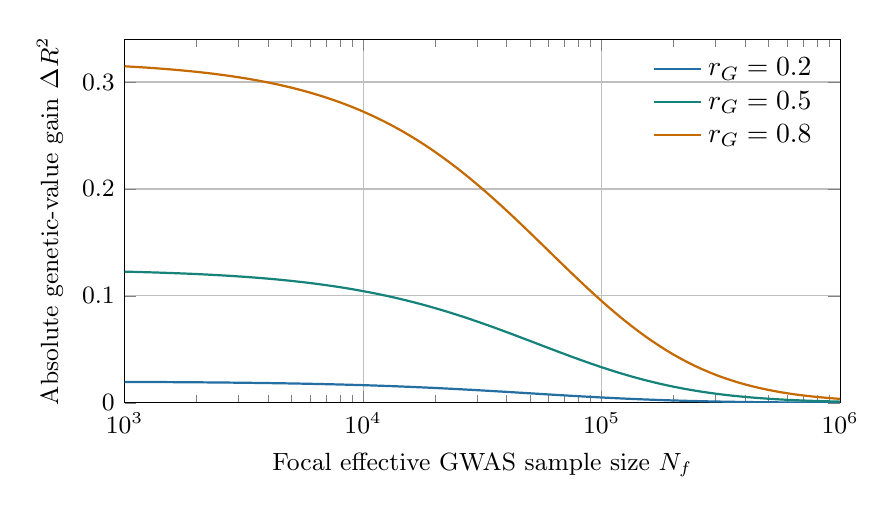
\begin{tikzpicture}
\begin{axis}[
  width=0.88\linewidth,height=62mm,
  xmode=log, xmin=1000,xmax=1000000,
  ymin=0,ymax=0.34,
  xlabel={Focal effective GWAS sample size \(N_f\)},
  ylabel={Absolute genetic-value gain \(\Delta R^2\)},
  grid=major,
  legend style={draw=none,fill=none,at={(0.98,0.98)},anchor=north east},
  tick label style={font=\small},
  label style={font=\small}
]
\addplot[DeepBlue,thick,domain=1000:1000000,samples=100]
 {(0.04*0.5*(1/(1+x/100000))^2)/
  (1-0.04*0.5*(x/100000)/(1+x/100000))};
\addlegendentry{\(r_G=0.2\)}
\addplot[Teal,thick,domain=1000:1000000,samples=100]
 {(0.25*0.5*(1/(1+x/100000))^2)/
  (1-0.25*0.5*(x/100000)/(1+x/100000))};
\addlegendentry{\(r_G=0.5\)}
\addplot[Amber,thick,domain=1000:1000000,samples=100]
 {(0.64*0.5*(1/(1+x/100000))^2)/
  (1-0.64*0.5*(x/100000)/(1+x/100000))};
\addlegendentry{\(r_G=0.8\)}
\end{axis}
\end{tikzpicture}
\caption{Analytical two-score gain from \cref{eq:two-score-gain}. The
illustration fixes \(h_f^2=0.2\), \(M=20{,}000\), and auxiliary
\(R_k^2=0.5\), so \(x_f=N_f/100{,}000\). It is an equation plot, not an
empirical performance claim.}
\label{fig:gain}
\end{figure}

\section{Implemented methods}
\label{sec:methods}

\begin{figure}[H]
\centering
\resizebox{0.96\linewidth}{!}{%
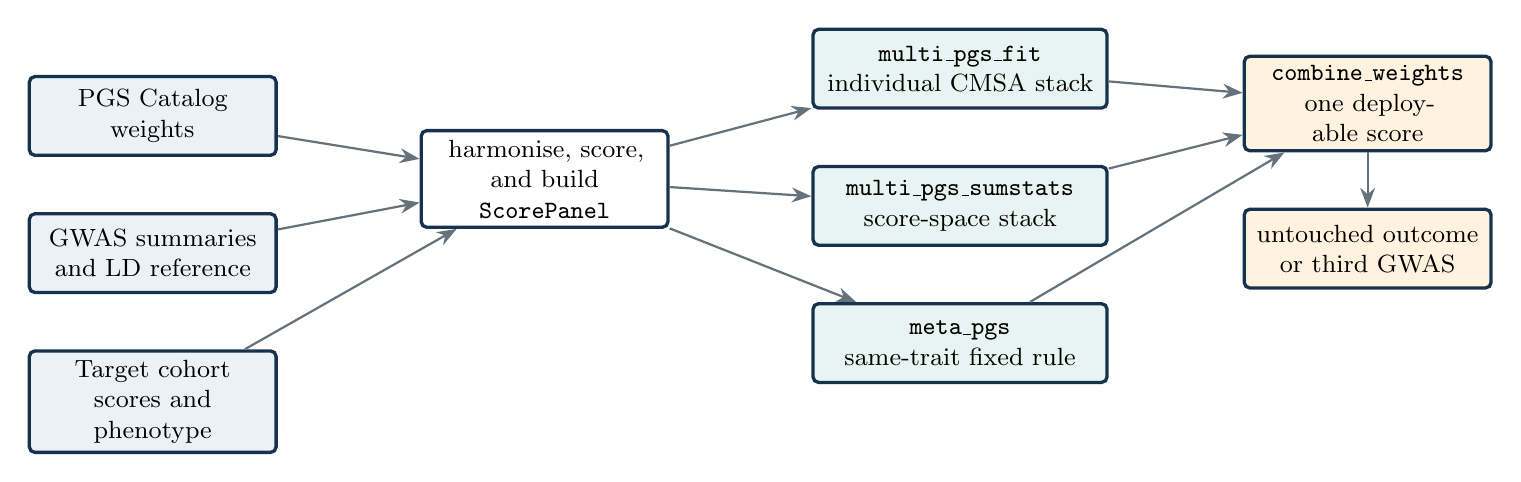
\begin{tikzpicture}[
  node distance=7mm and 7mm,
  box/.style={rounded corners=2pt,draw=DeepNavy,very thick,align=center,
              minimum height=10mm,text width=29mm,fill=white,font=\small},
  source/.style={box,fill=SoftBlue},
  method/.style={box,fill=SoftTeal,text width=35mm},
  output/.style={box,fill=SoftAmber},
  arr/.style={-{Stealth[length=2.5mm]},thick,draw=MidGray}
]
\node[source] (catalog) {PGS Catalog\\weights};
\node[source,below=of catalog] (gwas) {GWAS summaries\\and LD reference};
\node[source,below=of gwas] (cohort) {Target cohort\\scores and phenotype};
\node[box,right=18mm of catalog,yshift=-8mm] (panel)
 {harmonise, score,\\and build \code{ScorePanel}};
\node[method,right=18mm of panel,yshift=14mm] (individual)
 {\code{multi\_pgs\_fit}\\individual CMSA stack};
\node[method,below=of individual] (summary)
 {\code{multi\_pgs\_sumstats}\\score-space stack};
\node[method,below=of summary] (meta)
 {\code{meta\_pgs}\\same-trait fixed rule};
\node[output,right=17mm of summary,yshift=13mm] (weights)
 {\code{combine\_weights}\\one deployable score};
\node[output,below=of weights] (evaluate)
 {untouched outcome\\or third GWAS};
\draw[arr] (catalog) -- (panel);
\draw[arr] (gwas) -- (panel);
\draw[arr] (cohort) -- (panel);
\draw[arr] (panel) -- (individual);
\draw[arr] (panel) -- (summary);
\draw[arr] (panel) -- (meta);
\draw[arr] (individual) -- (weights);
\draw[arr] (summary) -- (weights);
\draw[arr] (meta) -- (weights);
\draw[arr] (weights) -- (evaluate);
\end{tikzpicture}
}
\caption{End-to-end package workflow. The three combination routes solve
different information problems and are not interchangeable. Assessment data
must be untouched by component discovery, combination fitting, and tuning.}
\label{fig:workflow}
\end{figure}

\begin{table}[H]
\centering
\caption{Information and validation contract for the three fitting routes.}
\label{tab:method-contract}
\scriptsize
\begin{tabularx}{\linewidth}{@{}L{26mm}Y Y Y@{}}
\toprule
\textbf{Route} & \textbf{Learns from} & \textbf{Selection / tuning} &
\textbf{Valid assessment} \\
\midrule
\code{multi\_pgs\_fit} & Individual score matrix, target phenotype, optional
covariates & Inner CMSA choices inside outer folds; final coefficients average
fold-selected fits; nested heuristic may return the baseline &
Independent individuals who trained neither component scores nor the
combination \\
\code{multi\_pgs\_sumstats} & Target-GWAS cross-moments plus external LD
score Gram & Same moments, an independent second GWAS, or PUMAS-style
pseudo-splits & A third untouched GWAS or independent individual-level cohort;
tuning performance is not assessment \\
\code{meta\_pgs} & Same-trait scores plus effective sample sizes or expected
accuracies; target score correlations for decorrelation & No fitted tuning;
ridge only stabilises inversion & Independent target outcomes; simple
metadata-derived weights remain hypotheses until tested \\
\bottomrule
\end{tabularx}
\end{table}

\subsection{Individual-level penalised stacking}

Within each training fold, score columns are imputed and standardised. With
unpenalised covariates \(X\), the Gaussian or binomial elastic-net objective is
\begin{equation}
  \min_{b_0,\gamma,\theta}
  \frac{1}{2n}\,
  \mathcal L\!\left(y,b_0+X\gamma+Z\theta\right)
  +\lambda\sum_{k=1}^{q}p_k
  \left\{\alpha|\theta_k|
  +\frac{1-\alpha}{2}\theta_k^2\right\}.
  \label{eq:individual-objective}
\end{equation}
Covariates receive penalty factor zero. The Gaussian path uses covariance
updates; the binomial path uses IRLS with coordinate descent, following the
glmnet family of algorithms \cite{friedman2010}. For a standardised Gaussian
column with current partial score \(z_k^\star\), the coordinate update is
\begin{equation}
  \theta_k \leftarrow
  \frac{\operatorname{sign}(z_k^\star)
        (|z_k^\star|-\lambda\alpha p_k)_+}
       {G_{kk}+\lambda(1-\alpha)p_k}.
  \label{eq:coordinate-update}
\end{equation}

CMSA fits a path inside folds, selects a fold-specific model, and averages the
selected coefficient vectors \cite{prive2019}. \pkg{multipgs} adds a separate
nested outer-fold decision rule that falls back to the unpenalised baseline
when the apparent increment is insufficient. The null benchmark shows that
this is a pragmatic guard, not a calibrated hypothesis test: pure noise passed
in 7 of 30 runs at \(n=1000\) and 4 of 30 at \(n=5000\).

The averaged support is the union of fold supports. Consequently
\code{selected()} reports predictive weights, not causal traits, unique genetic
contributors, or stable feature-selection discoveries. In the checked
simulation, support recall is high (0.84--1.00 by regime) while precision is
only 0.09--0.20.

\subsection{Summary-statistic score-space stacking}

Let \(W_{\mathrm{LD}}\) contain component weights on the LD source's
standardised-genotype scale, \(D\) be its LD correlation matrix, and
\(W_{\mathrm{GWAS}}\) contain the same component scores on the GWAS source's
standardised-genotype scale. The sufficient moments are
\begin{equation}
  G_{\mathrm{raw}}=
    W_{\mathrm{LD}}^{\mathsf T} D W_{\mathrm{LD}},
  \qquad
  c_{\mathrm{raw}}=
    W_{\mathrm{GWAS}}^{\mathsf T}z .
  \label{eq:score-moments}
\end{equation}
Writing \(A=\operatorname{diag}
(\sqrt{\operatorname{diag}(G_{\mathrm{raw}})})\), the fitted coordinates use
\begin{equation}
  G=A^{-1}G_{\mathrm{raw}}A^{-1},
  \qquad
  c=A^{-1}c_{\mathrm{raw}} .
  \label{eq:standardized-moments}
\end{equation}
This is the same Gaussian objective as \cref{eq:individual-objective}, but in
the span of the supplied scores. At \(\alpha=1\), the lasso selects entire
component scores; it is inspired by the SNP-level lassosum quadratic
\cite{mak2017}, but is not SNP-level lassosum.

For a fixed coefficient vector, summary tuning evaluates
\begin{equation}
  \operatorname{MSE}(\theta)
    =\operatorname{var}(y)-2\theta^{\mathsf T}c
      +\theta^{\mathsf T}G\theta,
  \qquad
  \widetilde R^2(\theta)
    =\frac{(\theta^{\mathsf T}c)^2}
    {\operatorname{var}(y)\,\theta^{\mathsf T}G\theta}.
  \label{eq:summary-metrics}
\end{equation}
MSE, not squared correlation, selects the path because \Rtwo{} is blind to a
reversed predictor. An independent second GWAS can tune the path; a third is
still needed for assessment. PUMAS-style pseudo-splitting uses a
joint-Gaussian/CLT covariance approximation \cite{zhao2021}. In the committed
calibration, relative covariance error is 3.77\% for Gaussian and 10.99\% for
binary simulations.

\subsection{Training-free same-trait combination}

The simple rules standardise component scores and use
\begin{equation}
  w_k\propto\sqrt{N_{\mathrm{eff},k}}
  \quad\text{or}\quad
  w_k\propto\sqrt{\widehat R_k^2}.
  \label{eq:meta-simple}
\end{equation}
The first is a power-limited approximation sourced from pipeline code, not
from the Hansen et al. preprint. Under independent estimation errors, the
exact same-trait GLS direction is
\begin{equation}
  w_k\propto\frac{R_k}{1-R_k^2},
  \label{eq:meta-gls}
\end{equation}
so direct accuracy weighting is accurate only as every \(R_k\) approaches
zero. The decorrelated rule is
\begin{equation}
  w_\delta\propto(C+\delta I)^{-1}\rho.
  \label{eq:meta-decorrelated}
\end{equation}
Its algebra is exact under \cref{eq:index-optimum}, but small error in
\(\rho\) is amplified along low-eigenvalue directions of \(C\). Ridge reduces
that amplification only by moving the result back toward an undecorrelated
weighted sum. If only Daetwyler proxies are available, the checked real CAD
diagnostic supports \code{expected\_r2}, not \code{decorrelated}.

\subsection{Panel construction, deployment, and evaluation}

\code{panel\_from\_catalog} harmonises alleles and constructs scores in one
genotype pass. \code{panel\_from\_sumstats} fits component scores through
ldpred3. Identifier order, genome build, effect orientation, and
source-specific dosage standard deviation are part of the statistical
contract, not file-format trivia.

Combining component variant weights \(w_{jk}\) with raw-score coefficients
\(\beta_k\) produces the deployable effect
\begin{equation}
  \widetilde w_j=\sum_{k=1}^{q}w_{jk}\beta_k .
  \label{eq:combined-weights}
\end{equation}
The frozen scoring scale should be carried to new cohorts. Re-standardising
each cohort independently can change coefficients, calibration, and even the
meaning of a fixed threshold.

With covariates, \pkg{multipgs} reports the unnormalised increment
\begin{equation}
  R^2_{\mathrm{incremental}}
  =R^2_{\mathrm{covariates+score}}-R^2_{\mathrm{covariates}}.
  \label{eq:incremental-r2}
\end{equation}
The Albi\~nana paper instead divides this difference by
\(1-R^2_{\mathrm{covariates}}\) \cite{albinana2023}; absolute values are
therefore not identical even when relative comparisons share covariates.

For binary outcomes, with population prevalence \(\pi\), sample case fraction
\(p_s\), threshold \(t=\Phi^{-1}(1-\pi)\), density
\(\varphi(t)\), and \(i=\varphi(t)/\pi\), the implemented Lee transformation is
\begin{equation}
  C_{\mathrm{LT}}=
  \frac{[\pi(1-\pi)]^2}{\varphi(t)^2p_s(1-p_s)},
  \quad
  \vartheta=
  \frac{i(p_s-\pi)}{1-\pi}
  \left\{\frac{i(p_s-\pi)}{1-\pi}-t\right\},
  \quad
  R_L^2=
  \frac{C_{\mathrm{LT}}R_O^2}
       {1+C_{\mathrm{LT}}\vartheta R_O^2}.
  \label{eq:liability-r2}
\end{equation}
This metric depends on a stated prevalence assumption \cite{lee2012}.

\section{Empirical evidence in the repository}
\label{sec:evidence}

\subsection{Individual fitting: estimator sanity}

\begin{figure}[H]
\centering
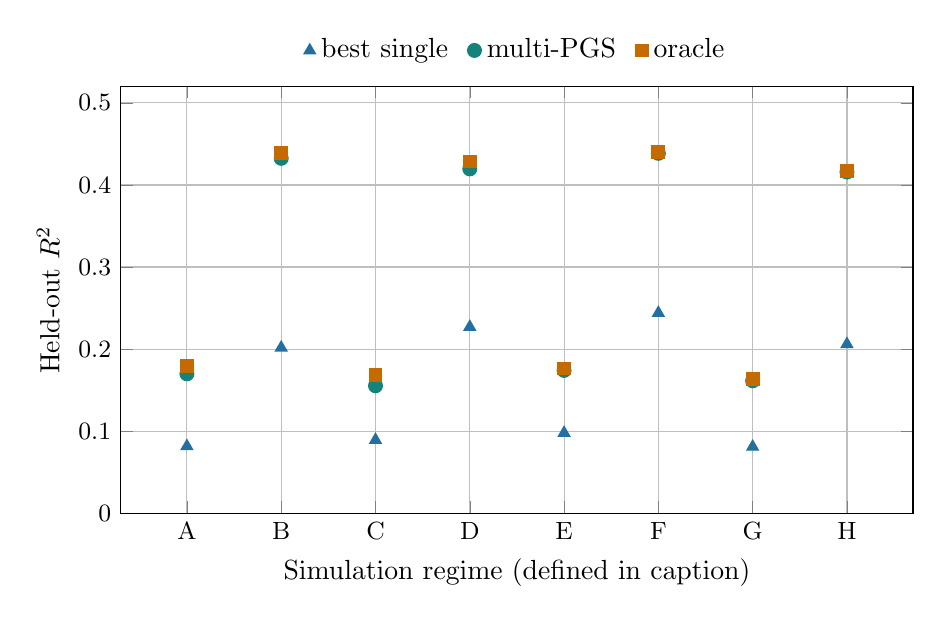
\begin{tikzpicture}
\begin{axis}[
  width=0.96\linewidth,height=70mm,
  symbolic x coords={A,B,C,D,E,F,G,H},
  xtick=data,
  ymin=0,ymax=0.52,
  ylabel={Held-out \(R^2\)},
  xlabel={Simulation regime (defined in caption)},
  grid=major,
  legend columns=3,
  legend style={draw=none,fill=none,at={(0.5,1.03)},anchor=south,
                /tikz/every even column/.append style={column sep=5pt}},
  tick label style={font=\small}
]
\addplot[only marks,mark=triangle*,mark size=2.4pt,DeepBlue]
 coordinates {(A,0.08169)(B,0.20177)(C,0.08925)(D,0.22703)
              (E,0.09785)(F,0.24406)(G,0.08094)(H,0.20603)};
\addlegendentry{best single}
\addplot[only marks,mark=*,mark size=2.5pt,Teal]
 coordinates {(A,0.16985)(B,0.43249)(C,0.15522)(D,0.41961)
              (E,0.17398)(F,0.43857)(G,0.16131)(H,0.41576)};
\addlegendentry{multi-PGS}
\addplot[only marks,mark=square*,mark size=2.3pt,Amber]
 coordinates {(A,0.17969)(B,0.43867)(C,0.16839)(D,0.42870)
              (E,0.17629)(F,0.44016)(G,0.16400)(H,0.41743)};
\addlegendentry{oracle}
\end{axis}
\end{tikzpicture}
\caption{Mean held-out \Rtwo{} over 30 seeds from
\protect\path{benchmarks/results/fit_accuracy_summary.csv}. Regimes A--D use
\(n=2000\), E--H use \(n=10{,}000\); A,B,E,F use \(q=50\), the others
\(q=200\); A,C,E,G use \(h^2=0.2\), the others \(h^2=0.5\). The multi-PGS
beats the training-selected best single score in all 240 raw replicates.
Because the simulated genetic value lies in the score span, this is an
estimator sanity check, not evidence of clinical efficacy.}
\label{fig:fit-accuracy}
\end{figure}

Across the eight regimes, mean uplift over the selected single score ranges
from 0.0660 to 0.2307 \Rtwo{}. Based on regime means, the fitted stack closes
83.4\%--99.2\% of the gap between the selected single score and the oracle.
The overall mean nested-CV minus held-out difference is \(-0.00230\), slightly
conservative in this simulation.

\subsection{Summary moments and LD-reference sensitivity}

With exact individual moments, the summary and individual standardised
coefficients correlate 0.999624 on average, and all compared held-out \Rtwo{}
values lie between 0.4973 and 0.4982. This supports the score-space identity
under the benchmark's strong-signal, small-\(q\) design.

\begin{figure}[H]
\centering
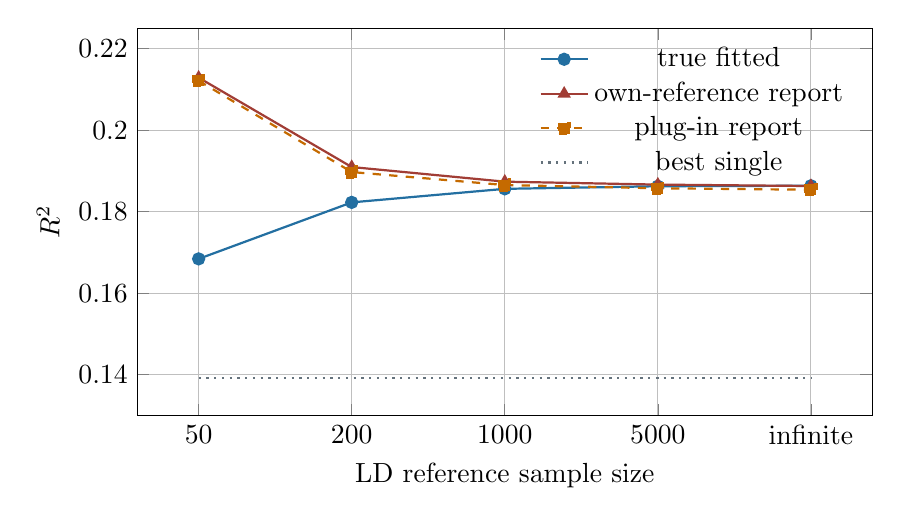
\begin{tikzpicture}
\begin{axis}[
  width=0.90\linewidth,height=65mm,
  symbolic x coords={50,200,1000,5000,infinite},
  xtick=data,
  ymin=0.13,ymax=0.225,
  xlabel={LD reference sample size},
  ylabel={\(R^2\)},
  grid=major,
  legend style={draw=none,fill=none,at={(0.98,0.98)},anchor=north east}
]
\addplot[DeepBlue,thick,mark=*]
 coordinates {(50,0.16842)(200,0.18228)(1000,0.18560)
              (5000,0.18624)(infinite,0.18636)};
\addlegendentry{true fitted}
\addplot[Critical,thick,mark=triangle*]
 coordinates {(50,0.21288)(200,0.19095)(1000,0.18736)
              (5000,0.18664)(infinite,0.18629)};
\addlegendentry{own-reference report}
\addplot[Amber,dashed,thick,mark=square*]
 coordinates {(50,0.21212)(200,0.18972)(1000,0.18653)
              (5000,0.18574)(infinite,0.18538)};
\addlegendentry{plug-in report}
\addplot[MidGray,dotted,thick]
 coordinates {(50,0.13918)(200,0.13918)(1000,0.13918)
              (5000,0.13918)(infinite,0.13918)};
\addlegendentry{best single}
\end{axis}
\end{tikzpicture}
\caption{Real-LD simulation from
\protect\path{real_ld_simulation_summary.csv}. At reference \(n=50\), true fitted
\Rtwo{} falls by 0.01795 relative to the infinite-reference result, while the
own-reference estimate is inflated by 0.04446 (26.4\% of true fitted
\Rtwo{}). Reporting bias is larger than the loss in the fitted predictor.}
\label{fig:ld-reference}
\end{figure}

\subsection{Overlap and decorrelation}

\begin{figure}[H]
\centering
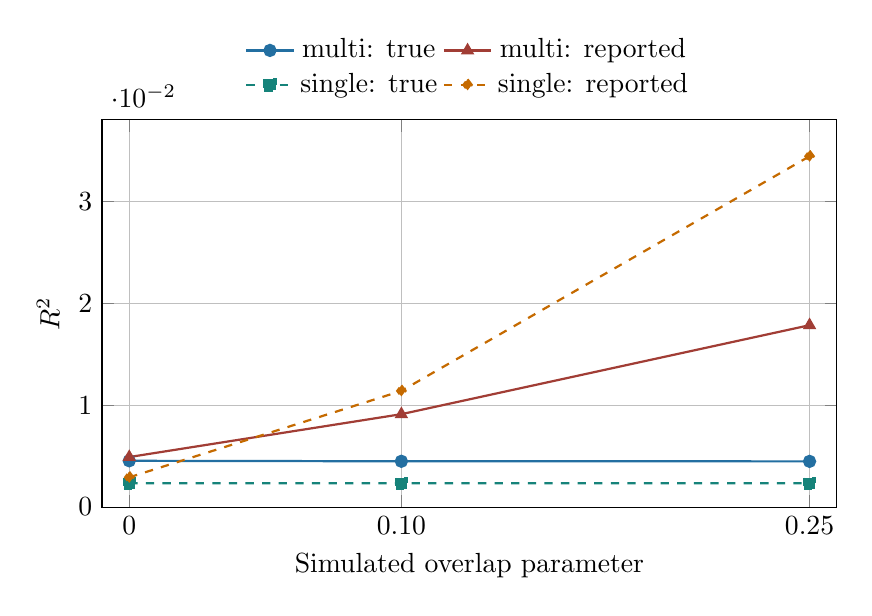
\begin{tikzpicture}
\begin{axis}[
  width=0.90\linewidth,height=65mm,
  xmin=-0.01,xmax=0.26,ymin=0,ymax=0.038,
  xtick={0,0.1,0.25},
  xticklabels={0,0.10,0.25},
  xlabel={Simulated overlap parameter},
  ylabel={\(R^2\)},
  grid=major,
  legend columns=2,
  legend style={draw=none,fill=none,at={(0.5,1.03)},anchor=south}
]
\addplot[DeepBlue,thick,mark=*]
 coordinates {(0,0.004539)(0.1,0.004493)(0.25,0.004484)};
\addlegendentry{multi: true}
\addplot[Critical,thick,mark=triangle*]
 coordinates {(0,0.004909)(0.1,0.009115)(0.25,0.017845)};
\addlegendentry{multi: reported}
\addplot[Teal,dashed,thick,mark=square*]
 coordinates {(0,0.002332)(0.1,0.002332)(0.25,0.002336)};
\addlegendentry{single: true}
\addplot[Amber,dashed,thick,mark=diamond*]
 coordinates {(0,0.002917)(0.1,0.011397)(0.25,0.034424)};
\addlegendentry{single: reported}
\end{axis}
\end{tikzpicture}
\caption{Known-overlap simulation from
\protect\path{overlap_inflation_summary.csv}. At overlap 0.10, reported-to-true
\Rtwo{} ratios are 2.03 for multi-PGS and 4.89 for the single score; at 0.25,
they are 3.98 and 14.73. Bivariate LDSC detected all 16 non-null runs and none
of eight null runs in this 109,590-variant design. This does not imply
universal LDSC power, but it refutes the absolute claim that no downstream
diagnostic can ever flag overlap.}
\label{fig:overlap}
\end{figure}

\begin{figure}[H]
\centering
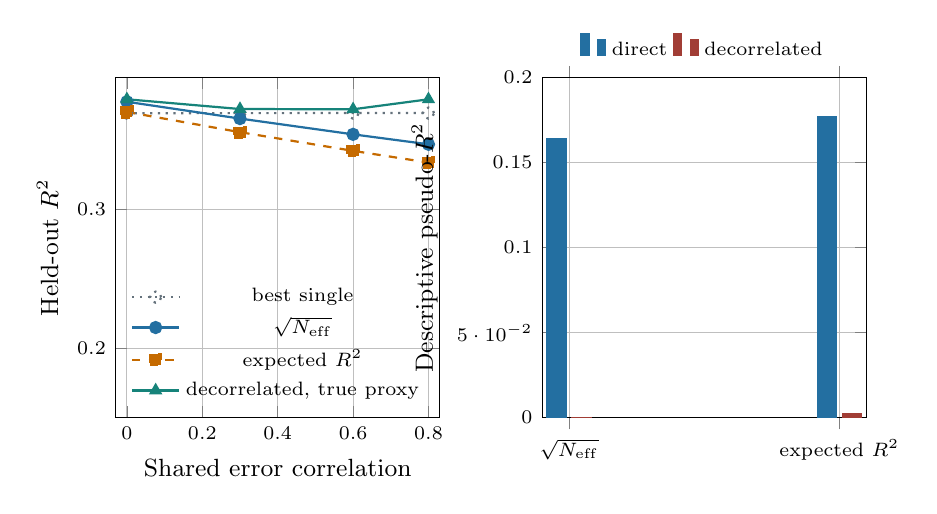
\begin{tikzpicture}
\begin{groupplot}[
  group style={group size=2 by 1,horizontal sep=13mm},
  width=0.47\linewidth,height=59mm,
  grid=major,
  tick label style={font=\scriptsize},
  label style={font=\small}
]
\nextgroupplot[
  xmin=-0.03,xmax=0.83,ymin=0.15,ymax=0.395,
  xlabel={Shared error correlation},
  ylabel={Held-out \(R^2\)},
  legend style={font=\scriptsize,draw=none,fill=none,at={(0.02,0.02)},
                anchor=south west}
]
\addplot[MidGray,dotted,thick,mark=o]
 coordinates {(0,0.36936)(0.3,0.36940)(0.6,0.36942)(0.8,0.36942)};
\addlegendentry{best single}
\addplot[DeepBlue,thick,mark=*]
 coordinates {(0,0.37758)(0.3,0.36547)(0.6,0.35411)(0.8,0.34693)};
\addlegendentry{\(\sqrt{N_{\rm eff}}\)}
\addplot[Amber,dashed,thick,mark=square*]
 coordinates {(0,0.37024)(0.3,0.35567)(0.6,0.34221)(0.8,0.33379)};
\addlegendentry{expected \(R^2\)}
\addplot[Teal,thick,mark=triangle*]
 coordinates {(0,0.37937)(0.3,0.37235)(0.6,0.37216)(0.8,0.37936)};
\addlegendentry{decorrelated, true proxy}

\nextgroupplot[
  ybar,bar width=7pt,
  symbolic x coords={sqrtN,expected},
  xtick=data,
  xticklabels={\(\sqrt{N_{\rm eff}}\),expected \(R^2\)},
  ymin=0,ymax=0.20,
  ylabel={Descriptive pseudo-\(R^2\)},
  legend style={font=\scriptsize,draw=none,fill=none,at={(0.5,1.02)},
                anchor=south,legend columns=2}
]
\addplot[fill=DeepBlue,draw=DeepBlue]
 coordinates {(sqrtN,0.16416)(expected,0.17729)};
\addlegendentry{direct}
\addplot[fill=Critical,draw=Critical]
 coordinates {(sqrtN,0.000167)(expected,0.002261)};
\addlegendentry{decorrelated}
\end{groupplot}
\end{tikzpicture}
\caption{Decorrelation behaves well when the simulation supplies the intended
accuracy structure (left, 30 seeds per point), but collapses with proxy
accuracies in the single checked 24-score CAD diagnostic (right). The right
panel is a contaminated regime-C score-space description, not external outcome
truth. Sources:
\protect\path{meta_rules_summary.csv} and
\protect\path{real_meta_rules_summary.csv}.}
\label{fig:decorrelation}
\end{figure}

\begin{table}[H]
\centering
\caption{Headline checked evidence, separated by evidence level.}
\label{tab:evidence}
\scriptsize
\begin{tabularx}{\linewidth}{@{}L{31mm}L{34mm}Y@{}}
\toprule
\textbf{Artifact} & \textbf{Result} & \textbf{What it supports - and does not} \\
\midrule
\path{fit_accuracy} & Multi-PGS wins 240/240 held-out simulations; uplift
0.0660--0.2307 & Supports estimator sanity when truth lies in the score span;
does not establish real-outcome or clinical superiority. \\
\path{null_gate} & Noise passes 11/60 runs overall & Shows the fallback is a
decision heuristic, not a significance test. \\
\path{sumstat_vs_individual} & coefficient correlation 0.999624; \Rtwo{}
0.4973--0.4982 & Supports exact-moment Gaussian equivalence in a small-\(q\),
strong-signal design. \\
\path{sumstat_calibration} & PUMAS covariance relative error 3.77\% Gaussian,
10.99\% binary & Quantifies approximation error; it does not validate
pseudotuning as assessment. \\
\path{real_ld_simulation} & reference \(n=50\) report inflation 0.04446 &
Demonstrates reference-induced optimism under real LD. \\
\path{overlap_inflation} & up to 3.98-fold multi-PGS and 14.73-fold single-score
inflation & Demonstrates overlap danger under a known covariance construction. \\
\path{real_meta_rules} & direct expected-\Rtwo{} proxy 0.17729 versus
decorrelated 0.002261 & Shows severe proxy sensitivity in one regime-C CAD
diagnostic; cannot rank methods externally. \\
\bottomrule
\end{tabularx}
\end{table}

\section{Technical review findings}
\label{sec:findings}

\subsection{Confirmed independent-tuning defect}

The helper \code{\_range\_basis\_from\_factor} normalises the columns of an
arbitrary covariance factor independently. Column normalisation does not make
an arbitrary factor orthogonal. Independent tuning then rescales this factor
by training score standard deviations and applies \(BB^{\mathsf T}\) as a
projection. The operation is a projection only if
\begin{equation}
  B^{\mathsf T}B=I
  \quad\Longrightarrow\quad
  P=BB^{\mathsf T},\;
  P^{\mathsf T}=P,\;
  P^2=P.
  \label{eq:orthogonal-projection}
\end{equation}
The implication's premise generally fails.

A public two-score reproduction uses the full-rank tuning Gram
\begin{equation}
  G_v=
  \begin{pmatrix}
    4 & 3\\
    3 & 9
  \end{pmatrix}.
  \label{eq:bug-gram}
\end{equation}
Because \(G_v\) is full rank, its range is all of \(\mathbb R^2\), so the
correct range projection is the identity. With unequal training and tuning
score scales, the implementation changes training \(c=(0.2,0.1)\) to
\((0.391198,0.004401)\) and logs discarded fractions of 0.95599 for both
training and tuning.

\begin{figure}[H]
\centering
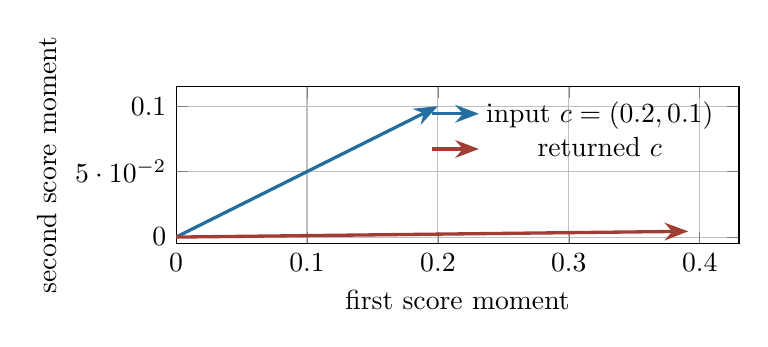
\begin{tikzpicture}
\begin{axis}[
  width=0.72\linewidth,height=57mm,
  xmin=0,xmax=0.43,ymin=-0.005,ymax=0.115,
  xlabel={first score moment},
  ylabel={second score moment},
  grid=major,
  axis equal image,
  legend style={draw=none,fill=none,at={(0.98,0.98)},anchor=north east}
]
\draw[-{Stealth[length=3mm]},very thick,DeepBlue]
  (axis cs:0,0) -- (axis cs:0.2,0.1);
\addlegendimage{DeepBlue,very thick,-{Stealth[length=3mm]}}
\addlegendentry{input \(c=(0.2,0.1)\)}
\draw[-{Stealth[length=3mm]},very thick,Critical]
  (axis cs:0,0) -- (axis cs:0.391198,0.004401);
\addlegendimage{Critical,very thick,-{Stealth[length=3mm]}}
\addlegendentry{returned \(c\)}
\end{axis}
\end{tikzpicture}
\caption{Independent-tuning counterexample. A projection onto the range of a
full-rank \(2\times2\) Gram must leave every vector unchanged. The large
rotation and rescaling therefore prove a correctness defect rather than a
numerical tolerance dispute.}
\label{fig:projection-bug}
\end{figure}

The simplest repair is to derive the independent-tuning basis directly from
\code{\_range\_basis(sel\_gram)}, or to compute a rank-revealing QR/SVD basis
for the scaled factor. Regression tests should assert orthonormality,
symmetry/idempotence, full-rank identity, scale invariance, and correct
rank-deficient behaviour.

\begin{longtable}{@{}L{15mm}L{39mm}L{48mm}L{54mm}@{}}
\caption{Prioritised review findings.}
\label{tab:findings}\\
\toprule
\textbf{Priority} & \textbf{Location} & \textbf{Finding and consequence} &
\textbf{Recommended action} \\
\midrule
\endfirsthead
\toprule
\textbf{Priority} & \textbf{Location} & \textbf{Finding and consequence} &
\textbf{Recommended action} \\
\midrule
\endhead
\finding{Critical}{High} &
\path{sumstat.py:1002-1012,1326-1338} &
Non-orthogonal factor columns are used as an orthonormal range basis.
Independent tuning can distort all moments even for full-rank tuning LD. &
Block the independent route; use an eigendecomposition or QR/SVD basis; add the
five regression tests described above. \\
\finding{Critical}{High} &
\path{README.md:125-132}; \path{guide.md:441-445} &
The showcased Daetwyler-to-\code{decorrelated} recipe contradicts code comments
and the checked CAD diagnostic, where \Rtwo{} falls 78-fold. &
Show \code{expected\_r2} for metadata proxies. Reserve decorrelation for
accurate, correctly oriented component accuracy and require external
assessment. \\
\finding{Amber}{Medium} &
\path{theory.md:175-190}; \path{algorithm.md:5-20} &
The objective is written on raw scores, while implementation penalises
fold-standardised coefficients. Penalty factors are misinterpreted under the
raw equation. &
Define \(Z,\theta,\beta\) as in \cref{eq:standardization} and write the objective
as \cref{eq:individual-objective}. \\
\finding{Amber}{Medium} &
\path{algorithm.md:299-343} &
Moment-derived in-sample quantities are called \emph{true} and an untracked
oracle table reports \Rtwo{} 0.542; the committed run is regime C. &
Replace with checked artifact values, label pseudo-\Rtwo{}, and store any
future oracle/ridge sweep in machine-readable results. \\
\finding{Amber}{Medium} &
\path{sumstat.py:1970-1998} &
\code{align\_to\_reference} promises standardised-genotype weights even when no
SD conversion is requested. Ignoring a warning can create plausible,
incorrect moments. &
Require explicit scale or make the raw/standardised return contract explicit
in both type and documentation. \\
\finding{Amber}{Medium} &
\path{stack.py:471-476}; \path{_coord.py:208-233,370-420} &
Several numerical controls are not validated and solvers expose no convergence
status. Invalid settings or exhausted iterations can silently return partial
paths. &
Validate public controls and report convergence/iteration counts per path
point. \\
\finding{Amber}{Medium} &
\path{README.md:82}; \path{stack.py:selected} &
Selected scores are described as traits that \emph{carried the signal}. CMSA
support is unstable and predictive, not causal. &
Describe largest nonzero standardised weights; prohibit causal or genetic
correlation interpretation. \\
\finding{Amber}{Medium} &
\path{benchmarks/README.md}; provenance JSON &
Several prose values are stale; three real-data files record ldpred3 0.3.1,
outside the current dependency range; no git or script hash is recorded. &
Generate prose tables from CSV, record git and script hashes, and regenerate or
clearly grandfather incompatible runs. \\
\finding{DeepBlue}{Low} &
\path{meta.py:324-332} &
\code{expected\_r2} accepts finite values above one despite its documented
\Rtwo{} meaning. &
Reject values outside \([0,1]\), or rename the argument as an arbitrary
positive proxy. \\
\bottomrule
\end{longtable}

\section{Documentation and reproducibility assessment}
\label{sec:documentation}

The documentation's strongest feature is its willingness to state operational
failure modes: target/discovery overlap, relatedness, ancestry mismatch,
genome-build alignment, tuning-versus-assessment separation, and liability
prevalence. The bibliography is extensive and documentation tests require
cited DOIs to appear in the annotated reference list.

The main weakness is traceability. Numerical claims are copied manually into
prose, some diagnostic values exist only in stdout, and benchmark provenance
does not identify the exact source commit or script hash. As a result, a
scientifically careful paragraph can still be numerically stale.

\begin{table}[H]
\centering
\caption{Reproducibility and validation matrix.}
\label{tab:reproducibility}
\scriptsize
\begin{tabularx}{\linewidth}{@{}L{30mm}Y Y@{}}
\toprule
\textbf{Area} & \textbf{Current strength} & \textbf{Material gap} \\
\midrule
Tests & 294 passing tests cover API contracts, alignment, fitting, numerical
identities, and failure cases. & No coverage metric; no benchmark execution in
CI; the independent-tuning bug lacks a full-rank unequal-scale test. \\
Benchmark records & Eleven producer scripts and 34 artifacts include raw
seed rows, summaries, commands, timestamps, versions, and many input hashes. &
Some prose numbers drift; several real runs use incompatible ldpred3 metadata;
git commit and script hash are absent. \\
Scientific scope & Simulations test null behaviour, exact moments, overlap,
real LD, and score-correlation rules. & No real individual-level outcome
benchmark, ancestry transfer, replicated binary accuracy study, or competing
stacker comparison. \\
Documentation tests & Internal paths, benchmark names, bibliography shape, and
DOI membership are checked. & Anchors, snippets, factual citation metadata, and
CSV-to-prose numerical consistency are not checked. \\
Distribution & README, Markdown docs, examples, tests, and benchmarks are
included in the source distribution. & Before this report, LaTeX/PDF artifacts
were absent from both source and wheel distributions; broad benchmark grafting
can also capture ignored local data in developer builds. \\
\bottomrule
\end{tabularx}
\end{table}

\section{Interpretation limits}
\label{sec:limits}

\begin{enumerate}
  \item \textbf{No causal interpretation.} Coefficients optimise prediction
  under correlation and penalisation. They do not estimate genetic
  correlations, mediation, or trait-specific causal contributions.
  \item \textbf{No automatic overlap cure.} Cross-validation inside a target
  cohort cannot remove discovery contamination shared by every fold.
  Bivariate LDSC or named-cohort metadata may flag overlap under favourable
  conditions, but exclusion by design is stronger.
  \item \textbf{No ancestry model.} Fitting weights in a target cohort does not
  repair discovery-score or LD-reference non-portability. Absolute risk and
  score means are particularly unsafe across ancestries.
  \item \textbf{Direction matters.} Squared correlation hides sign reversal,
  and the training-free expected-\Rtwo{} routes assume consistent positive
  trait orientation. Report signed correlation or calibration slope alongside
  \Rtwo{}.
  \item \textbf{No clinical calibration.} A high ranking metric is not a
  calibrated probability. Calibration intercept/slope, subgroup performance,
  decision utility, and an externally justified prevalence are separate
  requirements.
  \item \textbf{Conditional uncertainty.} The package bootstrap conditions on
  fixed component scores and their discovered weights; it does not propagate
  component-GWAS, LD-reference, or architecture-estimation uncertainty.
\end{enumerate}

\section{Recommended roadmap}
\label{sec:roadmap}

\begin{table}[H]
\centering
\caption{Recommended sequence of work after this review.}
\label{tab:roadmap}
\small
\begin{tabularx}{\linewidth}{@{}L{13mm}L{34mm}Y@{}}
\toprule
\textbf{Order} & \textbf{Work item} & \textbf{Acceptance criterion} \\
\midrule
1 & Fix independent tuning & Full-rank unequal-scale moments are unchanged;
projection is orthogonal and idempotent; scale-invariance and rank-deficient
tests pass. \\
2 & Correct high-impact guidance & README and guide no longer recommend
decorrelation from Daetwyler proxies; scale and support interpretations match
code. \\
3 & Make evidence self-checking & Report tables/figures and key docs are
generated or tested against CSV; every benchmark records git commit, script
hash, exact dependency revision, and external-input identities. \\
4 & Expose convergence & Public numerical controls are validated and every
solver result reports convergence and iteration exhaustion. \\
5 & Add outcome validation & Replicated real individual-level continuous and
binary outcomes, untouched assessment, ancestry strata, calibration, and at
least one comparator stacker. \\
\bottomrule
\end{tabularx}
\end{table}

\section{Conclusion}
\label{sec:conclusion}

\pkg{multipgs} has a coherent central idea: move a difficult multi-trait
genomic problem into a smaller space of component scores, then choose weights
using the information actually available. The selection-index derivation
explains when gains are possible; the individual and summary Gaussian
objectives explain how weights are learned; and the same-trait rules provide a
transparent fallback when phenotypes are unavailable.

The package is not ready to treat every route as equally mature. Individual
fitting has strong controlled simulation support but needs external outcomes.
Summary fitting has convincing moment checks but its independent-tuning route
has a confirmed correctness defect. Training-free decorrelation is an oracle
formula whose practical success depends on an accuracy vector the package
usually cannot know. Fixing that distinction in both code and prose is the
highest-value next step.

\begin{thebibliography}{99}

\bibitem{smith1936}
H. F. Smith.
\newblock A discriminant function for plant selection.
\newblock \emph{Annals of Eugenics}, 7(3):240--250, 1936.
\newblock \href{https://doi.org/10.1111/j.1469-1809.1936.tb02143.x}
{doi:10.1111/j.1469-1809.1936.tb02143.x}.

\bibitem{hazel1943}
L. N. Hazel.
\newblock The genetic basis for constructing selection indexes.
\newblock \emph{Genetics}, 28(6):476--490, 1943.
\newblock \href{https://doi.org/10.1093/genetics/28.6.476}
{doi:10.1093/genetics/28.6.476}.

\bibitem{daetwyler2008}
H. D. Daetwyler, B. Villanueva, and J. A. Woolliams.
\newblock Accuracy of predicting the genetic risk of disease using a
genome-wide approach.
\newblock \emph{PLoS ONE}, 3(10):e3395, 2008.
\newblock \href{https://doi.org/10.1371/journal.pone.0003395}
{doi:10.1371/journal.pone.0003395}.

\bibitem{friedman2010}
J. Friedman, T. Hastie, and R. Tibshirani.
\newblock Regularization paths for generalized linear models via coordinate
descent.
\newblock \emph{Journal of Statistical Software}, 33(1), 2010.
\newblock \href{https://doi.org/10.18637/jss.v033.i01}
{doi:10.18637/jss.v033.i01}.

\bibitem{mak2017}
T. S. H. Mak, R. M. Porsch, S. W. Choi, X. Zhou, and P. C. Sham.
\newblock Polygenic scores via penalized regression on summary statistics.
\newblock \emph{Genetic Epidemiology}, 41(6):469--480, 2017.
\newblock \href{https://doi.org/10.1002/gepi.22050}
{doi:10.1002/gepi.22050}.

\bibitem{prive2019}
F. Priv\'e, H. Aschard, and M. G. B. Blum.
\newblock Efficient implementation of penalized regression for genetic risk
prediction.
\newblock \emph{Genetics}, 212(1):65--74, 2019.
\newblock \href{https://doi.org/10.1534/genetics.119.302019}
{doi:10.1534/genetics.119.302019}.

\bibitem{zhao2021}
Z. Zhao, Y. Wu, J. Miao, Y. Song, X. Zhong, et al.
\newblock PUMAS: fine-tuning polygenic risk scores with GWAS summary
statistics.
\newblock \emph{Genome Biology}, 22:257, 2021.
\newblock \href{https://doi.org/10.1186/s13059-021-02479-9}
{doi:10.1186/s13059-021-02479-9}.

\bibitem{lee2012}
S. H. Lee, M. E. Goddard, N. R. Wray, and P. M. Visscher.
\newblock A better coefficient of determination for genetic profile analysis.
\newblock \emph{Genetic Epidemiology}, 36(3):214--224, 2012.
\newblock \href{https://doi.org/10.1002/gepi.21614}
{doi:10.1002/gepi.21614}.

\bibitem{albinana2023}
C. Albi\~nana, Z. Zhu, A. J. Schork, et al.
\newblock Multi-PGS enhances polygenic prediction by combining 937 polygenic
scores.
\newblock \emph{Nature Communications}, 14:4702, 2023.
\newblock \href{https://doi.org/10.1038/s41467-023-40330-w}
{doi:10.1038/s41467-023-40330-w}.

\bibitem{hansen2026}
O. S. Hansen, L. A. Rasmussen, E. M. Pedersen, et al.
\newblock Mapping genetic architecture of thousands of complex traits using
GWAS summary statistics.
\newblock \emph{Research Square}, version 1, 2026. Preprint; not peer reviewed.
\newblock \href{https://doi.org/10.21203/rs.3.rs-9415305/v1}
{doi:10.21203/rs.3.rs-9415305/v1}.

\end{thebibliography}

\appendix
\section{Artifact provenance}
\label{app:provenance}

\begin{table}[H]
\centering
\caption{Files used directly for quantitative statements and figures.}
\label{tab:artifact-provenance}
\scriptsize
\begin{tabularx}{\linewidth}{@{}L{56mm}Y@{}}
\toprule
\textbf{Repository artifact} & \textbf{Use in this report} \\
\midrule
\path{benchmarks/results/fit_accuracy.csv} and
\path{fit_accuracy_summary.csv} & Individual-fit held-out accuracy,
uncertainty, support, and CV calibration. \\
\path{benchmarks/results/null_gate.csv} and
\path{null_gate_summary.csv} & Pure-noise and signal fallback behaviour. \\
\path{benchmarks/results/sumstat_vs_individual_summary.csv} &
Individual/summary coefficient and held-out accuracy agreement. \\
\path{benchmarks/results/sumstat_calibration_summary.csv} &
Exact-moment identity and PUMAS covariance approximation error. \\
\path{benchmarks/results/real_ld_simulation_summary.csv} &
Real-LD reference-size sensitivity and reporting bias. \\
\path{benchmarks/results/overlap_inflation_summary.csv} &
Known-overlap accuracy inflation and LDSC diagnostic rate. \\
\path{benchmarks/results/meta_rules_summary.csv} &
Synthetic same-trait rule sensitivity over shared residual correlation. \\
\path{benchmarks/results/real_meta_rules_summary.csv} &
Single real CAD regime-C descriptive comparison. \\
\bottomrule
\end{tabularx}
\end{table}

Three real-data provenance records report ldpred3 0.3.1, whereas the reviewed
\path{pyproject.toml} requires ldpred3 0.4.5--0.4.x. These records may reflect
stale editable-install metadata or an unsupported runtime; either way, exact
environmental provenance is unresolved. This report therefore uses them as
diagnostics with explicit caveats, not as current-version validation.

\section{Independent-tuning reproduction}
\label{app:reproduction}

The defect in \cref{fig:projection-bug} is reproduced with public API inputs:
\begin{equation}
  W_{\mathrm{train}}=\operatorname{diag}(1,10),
  \quad
  z_{\mathrm{train}}=(0.2,0.01)^{\mathsf T},
  \quad
  W_v=\operatorname{chol}(G_v)^{\mathsf T},
  \quad
  z_v=(W_v^{\mathsf T})^{-1}(0.4,0.7)^{\mathsf T}.
  \label{eq:bug-inputs}
\end{equation}
Calling \code{multi\_pgs\_sumstats} with identity LD for both sources,
\code{tune="independent"}, and \code{ld\_shrinkage=0.1} returns the altered
training moment shown in \cref{fig:projection-bug}. The correct full-rank
projection is identity regardless of the shrinkage used later in the fitted
quadratic.

\end{document}
